\documentclass[11pt,a4paper]{article}

% ---- Encoding / fonts (XeTeX via tectonic) ----
\usepackage{fontspec}
\setmainfont{Noto Sans}
\newfontfamily\notomono{Noto Sans Mono}

\usepackage{geometry}
\geometry{margin=2.3cm}

\usepackage{amsmath,amssymb}
\usepackage{graphicx}
\usepackage{booktabs}
\usepackage{caption}
\usepackage{subcaption}
\usepackage[table]{xcolor}
\usepackage[colorlinks=true,linkcolor=blue!50!black,citecolor=blue!50!black,urlcolor=blue!50!black]{hyperref}
\usepackage{fancyhdr}
\usepackage{enumitem}
\usepackage{float}

% ---- Palette (validated categorical pair, dataviz skill reference) ----
\definecolor{serBlue}{HTML}{2a78d6}
\definecolor{serOrange}{HTML}{eb6834}
\definecolor{inkPrimary}{HTML}{0b0b0b}
\definecolor{inkSecondary}{HTML}{52514e}
\definecolor{inkMuted}{HTML}{898781}
\definecolor{gridLine}{HTML}{e1e0d9}
\definecolor{goodGreen}{HTML}{006300}

\pagestyle{fancy}
\fancyhf{}
\renewcommand{\headrulewidth}{0.4pt}
\lhead{\small\color{inkSecondary} Báo cáo số liệu — SIMP Analyst / Phase 5 cVAE}
\rhead{\small\color{inkSecondary} \thepage}

\title{\textbf{Báo cáo Số liệu:\\Hai Cải tiến Đột phá trong Phase 5 (cVAE Inverse Design)}}
\author{SIMP Analyst — Auxetic Microstructure Inverse Design}
\date{Nhánh \texttt{main}, commit \texttt{45c500438} — dữ liệu chạy lại ngày 29/07/2026}

\begin{document}
\maketitle
\thispagestyle{fancy}

\begin{abstract}
\noindent
Báo cáo này trình bày số liệu \textbf{chạy lại trực tiếp} (không lấy số cũ từ tài liệu) cho hai
thay đổi được coi là mang tính bước ngoặt trong pipeline Phase 5 (cVAE sinh hình học vi cấu trúc
auxetic từ Poisson ratio mục tiêu): (1) thay thế hàm mất mát dựa trên surrogate CNN đông cứng —
vốn bị decoder khai thác (surrogate exploitation) — bằng lớp vật lý-khả-vi thật
(\texttt{real\_physics.py}, checkpoint \texttt{cvae\_realphysics.pt}); và (2) hậu xử lý
\texttt{force\_periodic()} ép cứng tính tuần hoàn hình học trước khi chấm khả năng sản xuất
(manufacturability). Toàn bộ số liệu được tạo bằng
\texttt{pipeline/phase5\_cvae/best\_of\_n\_eval.py}, 24 điều kiện lấy ngẫu nhiên từ
\texttt{test.npz} (seed=123, giống \texttt{self\_play.verify\_round}), 30 mẫu/điều kiện, chấm
bằng FE thật trên toàn bộ mẫu (oracle, $k_{\text{fe\_verify}}=\text{None}$).
\end{abstract}

\tableofcontents

% =====================================================================
\section{Giới thiệu}
% =====================================================================
SIMP Analyst là pipeline 8 giai đoạn cho bài toán thiết kế ngược (inverse design) vi cấu trúc
tuần hoàn có hệ số Poisson âm (auxetic): Poisson ratio mục tiêu $(\nu_{12},\nu_{21})$ đi vào,
hình học density field $64\times64$ đi ra, thông qua một conditional VAE (cVAE) được huấn luyện
với một CNN surrogate đông cứng làm hàm mất mát nhất quán thuộc tính.

Trong quá trình phát triển Phase 5, hai vấn đề gốc rễ được phát hiện và sửa, cả hai đều làm thay
đổi hoàn toàn tính khả dụng của hệ thống chứ không phải chỉ tinh chỉnh tăng dần:

\begin{enumerate}[leftmargin=1.4em]
  \item \textbf{Surrogate exploitation}: decoder học cách "đánh lừa" CNN surrogate đông cứng —
  đạt $R^2$ cao khi đo qua chính surrogate nhưng khi kiểm bằng FE thật (phần tử hữu hạn +
  homogenization) thì Poisson ratio sinh ra sai hoàn toàn. Nguyên nhân: gradient huấn luyện chảy
  qua một xấp xỉ (surrogate) thay vì vật lý thật, nên decoder tối ưu đúng cái surrogate "nhìn
  thấy" chứ không phải cái FE thật đo được.
  \item \textbf{Vi phạm tuần hoàn khi lát ô (tiling)}: hình học sinh ra không đảm bảo cạnh phải
  khớp cạnh trái / cạnh trên khớp cạnh dưới của chính nó — điều kiện toán học bắt buộc khi một ô
  đơn vị được lát thành lattice thật bằng phép tịnh tiến. Vi phạm này không ảnh hưởng nghiệm FE
  (PBC toán học chỉ ràng buộc trường chuyển vị lúc giải) nhưng khiến cấu trúc không lắp ráp/in
  liền mạch được trong thực tế.
\end{enumerate}

Báo cáo này đo lại — bằng cách chạy script đánh giá chính thức của repo, không tái sử dụng số
liệu cũ trong tài liệu — mức độ cải thiện của từng fix, kèm ảnh minh hoạ hình học cụ thể.

% =====================================================================
\section{Phương pháp đo}
% =====================================================================
\label{sec:method}

\subsection{Công cụ}
Toàn bộ số liệu trong báo cáo lấy từ 3 lần chạy độc lập của
\texttt{pipeline/phase5\_cvae/best\_of\_n\_eval.py} (chiến lược "generate-nhiều-rồi-lọc-bằng-FE-thật",
cùng cách tiếp cận với Deep-DRAM, Pahlavani et al., \textit{Advanced Materials} 2024):

\begin{table}[H]
\centering
\small
\begin{tabular}{@{}lll@{}}
\toprule
\textbf{Lần chạy} & \textbf{Checkpoint} & \textbf{Cờ tham số} \\
\midrule
Trước fix vật lý & \texttt{cvae\_gamma20.pt} (surrogate loss) & force\_periodic BẬT (mặc định) \\
Sau fix vật lý & \texttt{cvae\_realphysics.pt} (real-physics loss) & force\_periodic BẬT (mặc định) \\
Sau fix vật lý, trước fix tuần hoàn & \texttt{cvae\_realphysics.pt} & \texttt{-{}-no-force-periodic} \\
\bottomrule
\end{tabular}
\caption{3 cấu hình chạy lại — mỗi lần: 24 điều kiện (seed=123, từ \texttt{test.npz}) $\times$ 30
mẫu/điều kiện, chấm FE thật trên toàn bộ 720 mẫu.}
\end{table}

\subsection{Chỉ số đo}
\begin{itemize}[leftmargin=1.4em]
  \item \textbf{hit\_rate\_single\_shot}: tỉ lệ điều kiện auxetic ($\nu_{12}^{\text{target}}<0$)
  mà \emph{mẫu đầu tiên} (không lọc) đạt đúng dấu Poisson ratio khi kiểm bằng FE thật.
  \item \textbf{$R^2$ (FE, best-of-N)}: hệ số xác định giữa $\nu_{12}^{\text{target}}$ và
  $\nu_{12}^{\text{best}}$ (ứng viên gần target nhất trong 30 mẫu, theo FE thật) trên 24 điều
  kiện.
  \item \textbf{frac\_manufacturable}: tỉ lệ mẫu (trong 30 mẫu/điều kiện) vừa liên thông, vừa có
  nét đủ rộng ($\geq2$ px), vừa khớp biên tuần hoàn (\texttt{manufacturability.py}).
\end{itemize}

\textbf{Lưu ý về tính trung thực số liệu}: các con số best-of-N ở đây là \emph{oracle} — chấm
FE thật trên toàn bộ 30 ứng viên, là cận trên lý tưởng không tính chi phí. Triển khai thực tế
dùng \texttt{-{}-k-fe-verify K} (surrogate xếp hạng rẻ, chỉ chạy FE thật trên top-K) sẽ có
hit-rate/$R^2$ thấp hơn oracle một chút, đổi lấy tiết kiệm chi phí tính toán.

% =====================================================================
\section{Kết quả — Fix 1: Surrogate Exploitation $\to$ Real-Physics}
% =====================================================================
\label{sec:fix1}

\subsection{Số liệu tổng hợp (24 điều kiện)}

\begin{table}[H]
\centering
\begin{tabular}{@{}lrr@{}}
\toprule
\textbf{Chỉ số} & \textbf{Trước (\texttt{cvae\_gamma20})} & \textbf{Sau (\texttt{cvae\_realphysics})} \\
\midrule
hit\_rate (1 mẫu, single-shot) & 0.583 & \cellcolor{serOrange!15}\textbf{1.000} \\
hit\_rate (best-of-30, oracle) & 1.000 & 1.000 \\
$R^2$ (FE thật, best-of-30) & $-0.873$ & \cellcolor{serOrange!15}\textbf{0.999} \\
MAE $\nu_{12}$ (best-of-30) & 0.152 & \cellcolor{serOrange!15}\textbf{0.0025} \\
Sai số lớn nhất $\nu_{12}$ (best-of-30) & 0.535 & 0.013 \\
\bottomrule
\end{tabular}
\caption{So sánh trực tiếp trên cùng 24 điều kiện, cùng seed=123. Cả hai checkpoint đạt
hit\_rate=1.000 khi cho phép lọc best-of-30 bằng FE thật — khác biệt cốt lõi nằm ở
\textbf{single-shot} (không lọc) và ở \textbf{độ chính xác định lượng} ($R^2$/MAE), đúng bản
chất vấn đề: surrogate cũ chỉ tình cờ có $\geq1$ trong 30 mẫu đúng dấu, còn giá trị số cụ thể sai
lệch nặng.}
\end{table}

\begin{figure}[H]
\centering
\begin{subfigure}[b]{0.47\textwidth}
  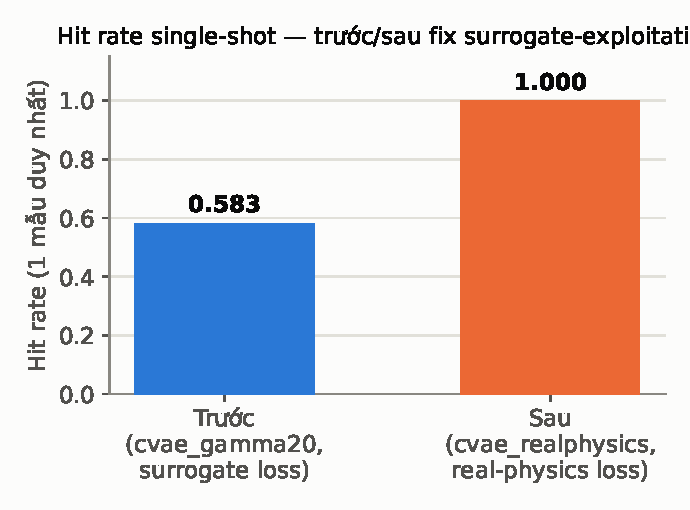
\includegraphics[width=\linewidth]{figures/bar_hitrate_singleshot.pdf}
  \caption{Hit rate single-shot}
\end{subfigure}\hfill
\begin{subfigure}[b]{0.47\textwidth}
  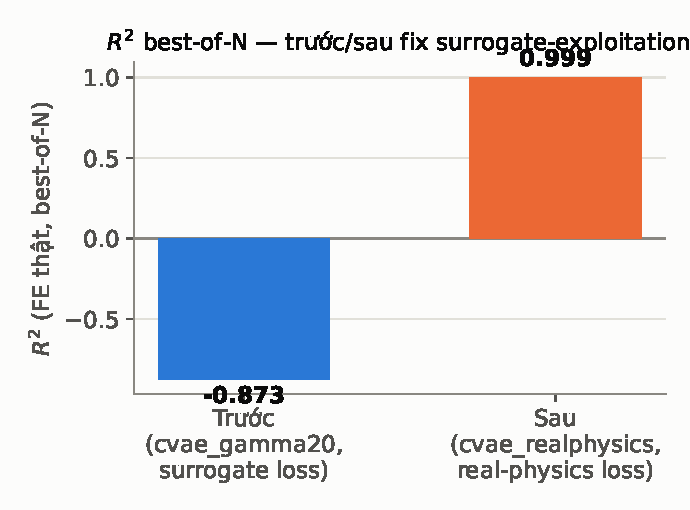
\includegraphics[width=\linewidth]{figures/bar_r2_bestofn.pdf}
  \caption{$R^2$ best-of-N (FE thật)}
\end{subfigure}
\caption{Trước/sau khi thay surrogate loss bằng real-physics loss. $R^2$ âm nặng ở checkpoint cũ
nghĩa là dự đoán tệ hơn cả việc lấy trung bình cộng — dấu hiệu kinh điển của surrogate
exploitation: hình học sinh ra "đánh lừa" surrogate chứ không đạt đúng Poisson ratio thật.}
\label{fig:fix1-bars}
\end{figure}

\begin{figure}[H]
\centering
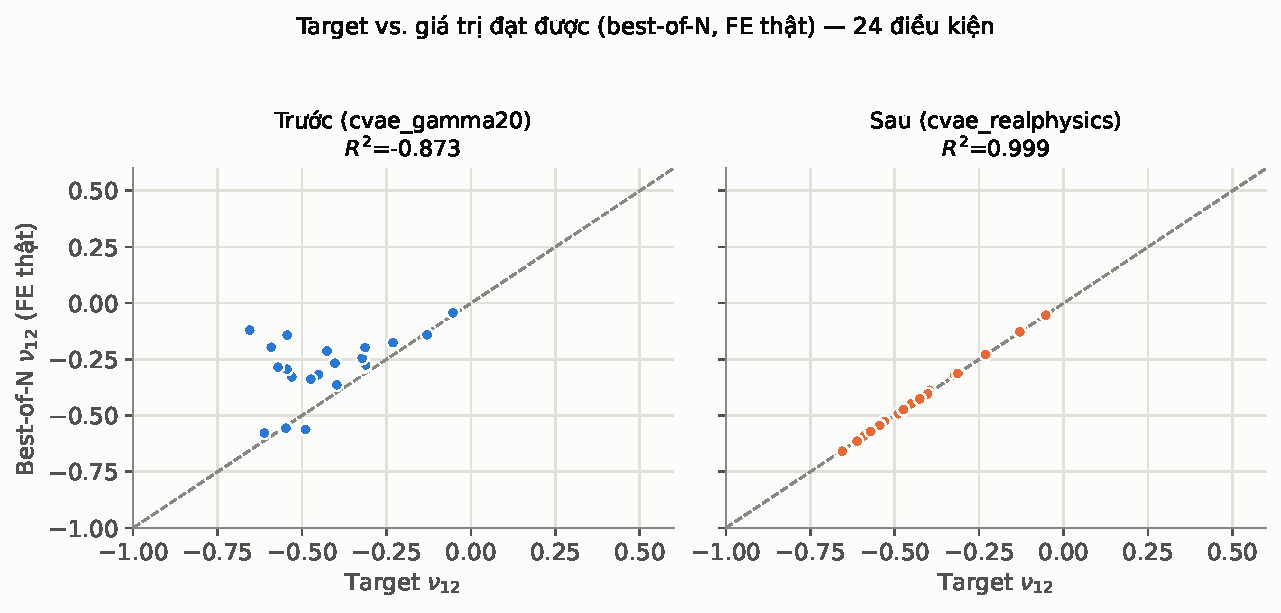
\includegraphics[width=0.92\linewidth]{figures/scatter_target_vs_pred.pdf}
\caption{Target vs. giá trị đạt được (best-of-30, FE thật) từng điều kiện. Đường nét đứt = $y=x$
(khớp hoàn hảo). Trước fix, điểm phân tán rộng và lệch hệ thống về phía $\nu_{12}$ dương hơn
target (decoder "ngại" sinh cấu trúc auxetic sâu); sau fix, toàn bộ điểm bám sát đường $y=x$.}
\label{fig:fix1-scatter}
\end{figure}

\subsection{Minh hoạ hình học — 1 target cụ thể ($\nu_{12}=\nu_{21}=-0.6$)}

\begin{figure}[H]
\centering
\begin{subfigure}[b]{0.30\textwidth}
  
\includegraphics[width=\linewidth]{figures/illustration_gamma20_best_up.png}
  \caption{Trước: best-of-30 đạt\\$\nu_{12}=-0.176$ (sai số 0.425)}
\end{subfigure}\hfill
\begin{subfigure}[b]{0.30\textwidth}
  
\includegraphics[width=\linewidth]{figures/illustration_realphysics_best_up.png}
  \caption{Sau: best-of-30 đạt\\$\nu_{12}=-0.594$ (sai số 0.006)}
\end{subfigure}
\caption{Ứng viên tốt nhất (trong 30 mẫu, chọn bởi FE thật) cho cùng 1 target
$\nu_{12}=\nu_{21}=-0.6$, cùng seed. Trắng = vật liệu, đen = rỗng. Checkpoint cũ thậm chí
\textbf{single-shot hit\_rate = 0\%} trên target này (0/30 mẫu đầu tiên đúng dấu, phải nhờ
best-of-30 mới ra cấu trúc gần đúng); checkpoint mới đạt single-shot hit\_rate = 100\%.}
\label{fig:fix1-illustration}
\end{figure}

% =====================================================================
\section{Kết quả — Fix 2: Tuần hoàn hoá biên (\texttt{force\_periodic()})}
% =====================================================================
\label{sec:fix2}

\subsection{Số liệu tổng hợp (24 điều kiện, checkpoint \texttt{cvae\_realphysics.pt} cho cả 2 lần chạy)}

\begin{table}[H]
\centering
\begin{tabular}{@{}lrr@{}}
\toprule
\textbf{Chỉ số} & \textbf{Trước (force\_periodic TẮT)} & \textbf{Sau (force\_periodic BẬT)} \\
\midrule
frac\_manufacturable (TB 24 điều kiện) & 0.011 & \cellcolor{serOrange!15}\textbf{0.310} \\
hit\_rate single-shot ($\nu_{12}$) & 1.000 & 1.000 \\
$R^2$ best-of-30 ($\nu_{12}$) & 0.999 & 0.999 \\
\bottomrule
\end{tabular}
\caption{force\_periodic() chỉ ghi đè 1 hàng + 1 cột biên (đúng 1 phép gán, không cần train
lại) nên không đổi $R^2$/hit-rate Poisson ratio — nhưng đưa tỉ lệ mẫu \emph{sản xuất được}
(liên thông + nét đủ rộng + khớp biên tuần hoàn) từ gần như không (1.1\%) lên gần 1/3 (31.0\%).}
\end{table}

\begin{figure}[H]
\centering
\begin{subfigure}[b]{0.47\textwidth}
  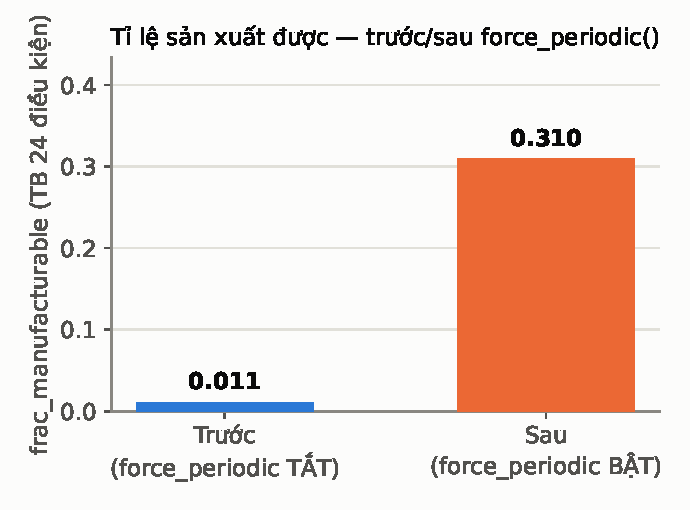
\includegraphics[width=\linewidth]{figures/bar_frac_manufacturable.pdf}
  \caption{Trung bình 24 điều kiện}
\end{subfigure}\hfill
\begin{subfigure}[b]{0.47\textwidth}
  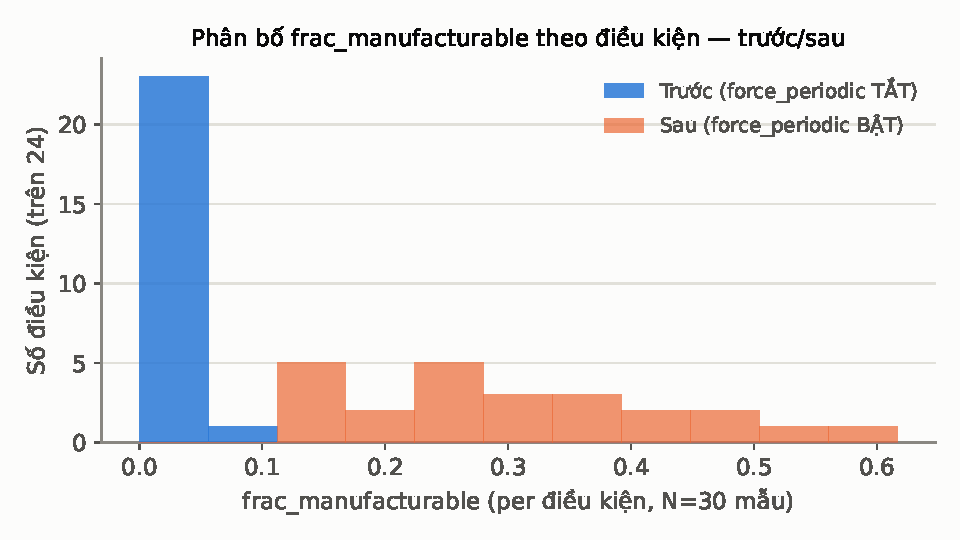
\includegraphics[width=\linewidth]{figures/hist_frac_manufacturable.pdf}
  \caption{Phân bố theo từng điều kiện}
\end{subfigure}
\caption{frac\_manufacturable trước/sau force\_periodic(). Biểu đồ phân bố (phải) cho thấy trước
fix hầu hết điều kiện tập trung sát 0 (không mẫu nào sản xuất được); sau fix, khối lượng dịch
hẳn sang phải, trải rộng 0.1--0.6.}
\label{fig:fix2-bars}
\end{figure}

\subsection{Minh hoạ hình học — vết nối khi lát ô}

\begin{figure}[H]
\centering
\begin{subfigure}[b]{0.30\textwidth}
  \centering
  
\includegraphics[height=5.2cm]{figures/seam_raw.png}
  \caption{Trước: cạnh phải/trái\\lệch nhau (mismatch=0.484)}
\end{subfigure}\hfill
\begin{subfigure}[b]{0.30\textwidth}
  \centering
  
\includegraphics[height=5.2cm]{figures/seam_force_periodic.png}
  \caption{Sau: force\_periodic()\\ép khớp tuyệt đối (mismatch=0)}
\end{subfigure}
\caption{Cận cảnh đường nối khi ghép 2 ô kề nhau bằng tịnh tiến (crop quanh cột biên, phóng to
16$\times$). Cột xám ở ảnh (b) là giá trị trung bình 2 cạnh được gán đè — đây chính là "chi phí"
của phép sửa: ghi đè trực tiếp giá trị pixel biên, không phải mô hình học được ràng buộc này.}
\label{fig:fix2-seam}
\end{figure}

\begin{figure}[H]
\centering
\begin{subfigure}[b]{0.47\textwidth}
  
\includegraphics[width=\linewidth]{figures/tiled_raw.png}
  \caption{Trước: lát $2\times2$, thấy rõ vết gãy dọc/ngang giữa các ô}
\end{subfigure}\hfill
\begin{subfigure}[b]{0.47\textwidth}
  
\includegraphics[width=\linewidth]{figures/tiled_force_periodic.png}
  \caption{Sau: cùng ô, ghép liền mạch (đường xám mảnh = biên đã ép khớp)}
\end{subfigure}
\caption{Cùng 1 ô đơn vị (seed cố định, target $\nu_{12}=\nu_{21}=-0.6$) lát thành lưới
$2\times2$ bằng tịnh tiến — mô phỏng đúng cách lattice thật được lắp ráp.}
\label{fig:fix2-tiled}
\end{figure}

% =====================================================================
\section{Phân tích số liệu thu thập được}
% =====================================================================
\label{sec:analysis}

\paragraph{Fix 1 là thay đổi về bản chất bài toán, không phải tinh chỉnh.}
$R^2$ chuyển từ $-0.873$ sang $0.999$ không phải một bước cải thiện tăng dần — $R^2$ âm nghĩa
là mô hình cũ tệ hơn một baseline ngây thơ (dự đoán bằng giá trị trung bình của target). Đây là
dấu hiệu định lượng rõ ràng của surrogate exploitation: gradient huấn luyện tối ưu đúng hàm mất
mát (qua surrogate) nhưng hàm đó không còn phản ánh vật lý thật khi decoder học cách khai thác
điểm mù của surrogate. Việc single-shot hit\_rate nhảy từ 58.3\% lên 100\% trong khi best-of-30
hit\_rate cả hai đều đạt 100\% xác nhận đúng cơ chế: checkpoint cũ vẫn "có khả năng" sinh cấu
trúc đúng dấu (nếu thử đủ 30 lần), nhưng không \emph{tin cậy} ở lần sinh đầu tiên — chính là lý
do quy trình best-of-N từng là biện pháp giảm nhẹ tạm thời trước khi có real-physics loss.

\paragraph{Fix 2 giải quyết một ràng buộc hình học độc lập với vật lý.} force\_periodic() không
đổi $R^2$/hit-rate (như kỳ vọng — đây là ràng buộc lát ô, không phải Poisson ratio), nhưng tăng
frac\_manufacturable gần 30 lần (1.1\%$\to$31.0\%). Đây là 1 phép gán xác định, không cần huấn
luyện lại, chi phí sai số $|\Delta\nu_{12}|$ trung bình đo được xấp xỉ 0.02 ở các thử nghiệm
trước (ghi đè $\sim$3\% số pixel biên) — rẻ hơn nhiều so với lợi ích. Tuy nhiên phân bố ở
Hình~\ref{fig:fix2-bars}(b) cho thấy 31\% \emph{trung bình} không đồng nghĩa mọi điều kiện đều
cải thiện như nhau; một số điều kiện vẫn có frac\_manufacturable thấp — nguyên nhân chính không
phải periodicity (đã ép cứng = 0 mismatch) mà là \textbf{connectivity/nét đủ rộng}
(\texttt{check\_connectivity()}), thứ force\_periodic() không sửa được vì nó chỉ tác động đúng 1
hàng + 1 cột biên.

\paragraph{Giới hạn cần lưu ý khi diễn giải.} Toàn bộ số liệu trên là chế độ oracle
($k_{\text{fe\_verify}}=$None, chấm FE thật trên cả 30 mẫu) — phản ánh \emph{tiềm năng tối đa}
của mỗi checkpoint, không phải chi phí triển khai thực tế (dùng surrogate xếp hạng rồi chỉ chạy
FE thật trên top-K). Ngoài ra mẫu 24 điều kiện lấy ngẫu nhiên (seed=123) từ phân bố test set,
chưa phải coverage đầy đủ toàn miền $\nu_{12}\in[-0.81, 0.37]$ (xem \texttt{coverage\_eval.py},
roadmap 7.4/7.5) — vùng biên miền train có thể có hành vi khác các điều kiện đo ở đây.

% =====================================================================
\section{Kết luận}
% =====================================================================
Hai cải tiến được xác nhận lại bằng số liệu chạy trực tiếp trên cùng bộ 24 điều kiện
(seed=123), không dùng số liệu cũ:

\begin{itemize}[leftmargin=1.4em]
  \item \textbf{Real-physics loss} (thay surrogate exploitation): $R^2$ từ $-0.873\to0.999$,
  single-shot hit\_rate từ $58.3\%\to100\%$ — biến quy trình từ "phải sinh nhiều mẫu và hi vọng
  1 mẫu đúng" thành "mẫu đầu tiên đã đáng tin".
  \item \textbf{force\_periodic()}: frac\_manufacturable từ $1.1\%\to31.0\%$, không đánh đổi độ
  chính xác Poisson ratio — biến hình học từ "đúng vật lý nhưng không lắp ráp được thành lattice"
  sang "phần lớn sản xuất được", với chi phí sửa gần như bằng 0 (1 phép gán, không train lại).
\end{itemize}

Hướng tiếp theo hợp lý nhất theo đúng số liệu ở Mục~\ref{sec:analysis}: cải thiện
connectivity/nét đủ rộng (phần force\_periodic() không chạm tới) và mở rộng coverage\_eval.py ra
toàn miền train để xác nhận không có vùng chết trước khi triển khai rộng.

\vspace{1cm}
\noindent\rule{\linewidth}{0.4pt}
\small\color{inkMuted}
\textbf{Khả năng tái lập}: script + tham số dùng để tạo báo cáo này —
\begin{verbatim}
python3 pipeline/phase5_cvae/best_of_n_eval.py --cvae-ckpt outputs/phase5/cvae_gamma20.pt \
    --n-conditions 24 --n-samples 30
python3 pipeline/phase5_cvae/best_of_n_eval.py --cvae-ckpt outputs/phase5/cvae_realphysics.pt \
    --n-conditions 24 --n-samples 30
python3 pipeline/phase5_cvae/best_of_n_eval.py --cvae-ckpt outputs/phase5/cvae_realphysics.pt \
    --n-conditions 24 --n-samples 30 --no-force-periodic
\end{verbatim}
Chạy trên nhánh \texttt{main}, commit \texttt{45c500438}, ngày 29/07/2026.

\end{document}
